\documentclass[tikz,border=8pt]{standalone}
\begin{document}
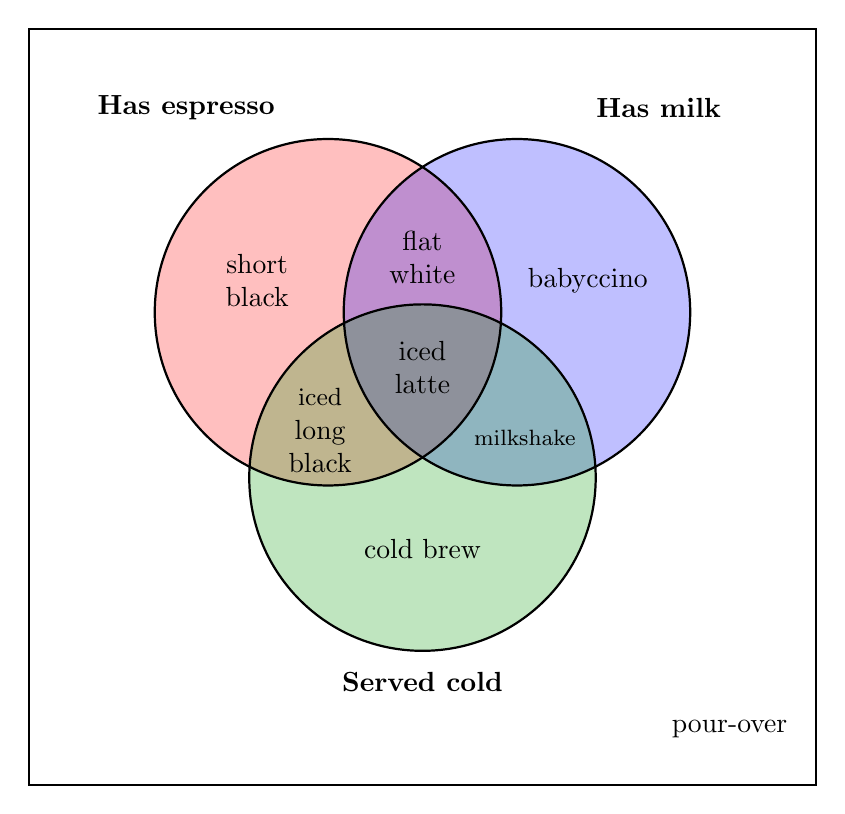
\begin{tikzpicture}
\draw[thick] (-5,-5) rectangle (5,4.6);
\begin{scope}
\fill[red,opacity=.25] (-1.2,1) circle (2.2);
\fill[blue,opacity=.25] (1.2,1) circle (2.2);
\fill[green!60!black,opacity=.25] (0,-1.1) circle (2.2);
\end{scope}
\draw[thick] (-1.2,1) circle (2.2);
\draw[thick] (1.2,1) circle (2.2);
\draw[thick] (0,-1.1) circle (2.2);
\node at (-3.0,3.6) {\bfseries Has espresso};
\node at (3.0,3.6) {\bfseries Has milk};
\node at (0,-3.7) {\bfseries Served cold};
\node[align=center] at (-2.1,1.4) {short\\black};
\node[align=center] at (2.1,1.4) {babyccino};
\node[align=center] at (0,-2.0) {cold brew};
\node[align=center] at (0,1.7) {flat\\white};
\node[align=center] at (-1.3,-0.5) {\small iced\\long\\black};
\node[align=center] at (1.3,-0.6) {\footnotesize milkshake};
\node[align=center] at (0,0.3) {iced\\latte};
\node at (3.9,-4.3) {pour-over};
\end{tikzpicture}
\end{document}
